\section{Evaluation}

\subsection{Text size importance in stylometry}

Figure~\ref{img:degradation} shows the importance of having texts large enough for a correct stylistic detection using distance between MFW vectors.

PAN16 dataset is a difficult dataset due to its small size, thus extracting reliable feature for each text to estimate each style is also a difficult task.
After multiple tests, the PAN @ CLEF 2016 dataset was not used further in this study due to its difficulty in finding reliable stylographic clues.

\begin{figure}
  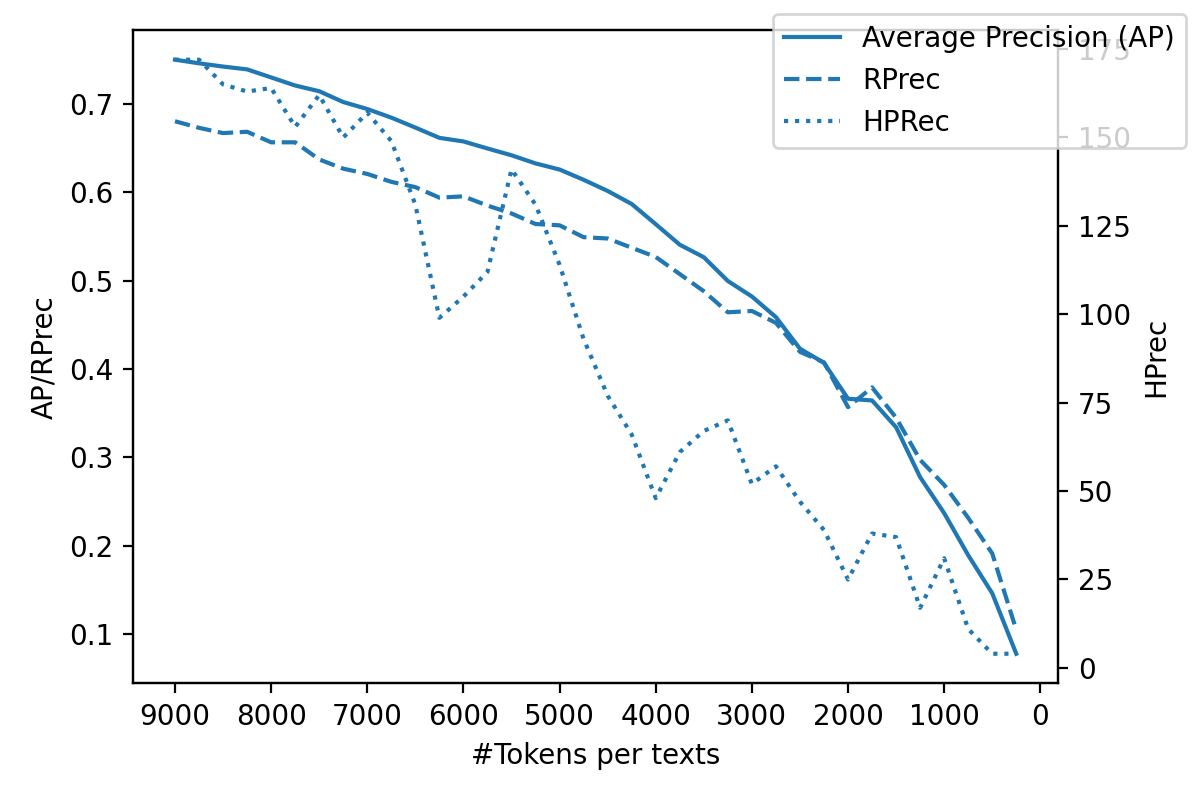
\includegraphics[width=\linewidth]{img/degradation.png}
  \caption{St-Jean ranks list evaluation on AP, RPrec and HPrec over the text size. Rank list computed using 500 MFW and the zscored-normalized cosine distance}
  \label{img:degradation}
\end{figure}


\subsection{Rank list evaluation}

Some of the definitions in this sections are an adapted version of the ones in~\cite{kocher_linking},~\cite{bcubed}.

\begin{definition}[Relevant link~\cite{kocher_linking}]
  A relevant link is a link in the relevant set.
  \begin{equation}
    relevant(l_i) =
    \begin{cases}
      1, & if\ l_i \in R \\
      0, & otherwise
    \end{cases}
  \end{equation}
\end{definition}

\begin{definition}[Precision@k~\cite{kocher_linking}]
  The precision@k is a function which take a integer k, with k < |L|
  \begin{equation}
    precision(k) = \frac{1}{k} \sum_{j=1}^{k} relevant(j)
  \end{equation}
\end{definition}

\begin{definition}[Average Precision (AP)]
  The mean over the precision@k each time a relevant link is retrieved.
  \begin{equation}
    AveragePrecision = \frac{1}{|R|} \sum_{j=1}^{|L|} precision(j) \cdot relevant(j)
  \end{equation}
\end{definition}

\begin{definition}[RPrec~\cite{kocher_linking}]
  The RPrec is the precision in the rank list at rank |R|.
  With R being the relevant set. (Not to be confused with the r ratio)
  \begin{equation}
    RPrec = precision(|R|)
  \end{equation}
\end{definition}

\begin{definition}[HPrec~\cite{kocher_linking}]
  The HPrec represent a maximal rank j in the rank list where the precision is still 100\%.
  This value is in the range [0 - |R|].
  0 means the first pair in the rank list is incorrect.
  |R| means every true links are ranked in the top part of the rank list.
  \begin{equation}
    HPrec = \max\{i \in \mathbf{N} | precision(i) = 1\}
  \end{equation}
\end{definition}

\subsection{Clustering evaluation}

\begin{definition}[Correctness~\cite{bcubed}]
  Let L(e) and C(e) be the category and the cluster of an element e.
  The correctness has a value of one if the two elements are in the both in the same cluster and has the same category OR both in a different cluster and a different category. ($A \Longleftrightarrow B \equiv (A \land B) \lor (\neg A \land \neg B)$)
  \begin{gather*}
    Correctness(e, e') = \\
    \begin{cases}
      1, & if (L(e) = L(e')) \Longleftrightarrow (C(e) = C(e'))\\
      0, & otherwise
    \end{cases}
  \end{gather*}
\end{definition}

\begin{definition}[Precision $BCubed$~\cite{bcubed}]
  The average of correctness for all elements on the average of all element such that their cluster is the same.
  \begin{equation}
    BCubed_{precision} = \text{Avg}_{e}[\text{Avg}_{e' C(e)=C(e')}[Correctness(e, e')]]
  \end{equation}
\end{definition}

\begin{definition}[Recall $BCubed$~\cite{bcubed}]
  The average of correctness for all elements on the average of all element such that their category is the same.
  \begin{equation}
    BCubed_{recall} = \text{Avg}_{e}[\text{Avg}_{e' L(e)=L(e')}[Correctness(e, e')]]
  \end{equation}
\end{definition}

\begin{definition}[$BCubed F_1$ Score~\cite{bcubed}]
  The harmonic mean between the $BCubed_{precision}$ and $BCubed_{recall}$
  \begin{equation}
    BCubed_{F_1} =
    2 \cdot \frac{BCubed_{precision} \cdot BCubed_{recall}}
    {BCubed_{precision} + BCubed_{recall}}
  \end{equation}
\end{definition}
